\documentclass{acm_proc_article-sp}

\begin{document}
%
% --- Author Metadata here ---
%\CopyrightYear{2007} % Allows default copyright year (20XX) to be over-ridden - IF NEED BE.
%\crdata{0-12345-67-8/90/01}  % Allows default copyright data (0-89791-88-6/97/05) to be over-ridden - IF NEED BE.
% --- End of Author Metadata ---

\title{Meme Tracker}
\subtitle{Social Network Generation and Ranking}
%
% You need the command \numberofauthors to handle the 'placement
% and alignment' of the authors beneath the title.
%
% For aesthetic reasons, we recommend 'three authors at a time'
% i.e. three 'name/affiliation blocks' be placed beneath the title.
%
% NOTE: You are NOT restricted in how many 'rows' of
% "name/affiliations" may appear. We just ask that you restrict
% the number of 'columns' to three.
%
% Because of the available 'opening page real-estate'
% we ask you to refrain from putting more than six authors
% (two rows with three columns) beneath the article title.
% More than six makes the first-page appear very cluttered indeed.
%
% Use the \alignauthor commands to handle the names
% and affiliations for an 'aesthetic maximum' of six authors.
% Add names, affiliations, addresses for
% the seventh etc. author(s) as the argument for the
% \additionalauthors command.
% These 'additional authors' will be output/set for you
% without further effort on your part as the last section in
% the body of your article BEFORE References or any Appendices.

\numberofauthors{3} %  in this sample file, there are a *total*
% of EIGHT authors. SIX appear on the 'first-page' (for formatting
% reasons) and the remaining two appear in the \additionalauthors section.
%
\author{
% You can go ahead and credit any number of authors here,
% e.g. one 'row of three' or two rows (consisting of one row of three
% and a second row of one, two or three).
%
% The command \alignauthor (no curly braces needed) should
% precede each author name, affiliation/snail-mail address and
% e-mail address. Additionally, tag each line of
% affiliation/address with \affaddr, and tag the
% e-mail address with \email.
%
% 1st. author
\alignauthor
Eshwaran Vijaya Kumar\\
       \affaddr{Dept. of Electrical \& Computer Engineering}\\
       \affaddr{The University of Texas at Austin}\\
       \email{eshwaran@utexas.edu}
       \alignauthor
Saral  Jain\\
   \affaddr{Dept. of Computer Science}\\
       \affaddr{The University of Texas at Austin}\\
       \email{saral@cs.utexas.edu}
        \alignauthor
       Prateek Maheshwari \\
  \affaddr{Dept. of Computer Science}\\
  \affaddr{The University of Texas at Austin}\\
  \email{prateekm@utexas.edu}
}


% There's nothing stopping you putting the seventh, eighth, etc.
% author on the opening page (as the 'third row') but we ask,
% for aesthetic reasons that you place these 'additional authors'
% in the \additional authors block, viz.
\date{02 November 2011}
% Just remember to make sure that the TOTAL number of authors
% is the number that will appear on the first page PLUS the
% number that will appear in the \additionalauthors section.

\maketitle
% A category with the (minimum) three required fields
\category{H.4}{Information Systems Applications}{Machine Learning, Text Mining}
%A category including the fourth, optional field follows...

\terms{Machine Learning, Text Mining, Mapreduce}

\section{Introduction}
The term meme was first coined by the British evolutionary biologist Richard Dawkins in \cite{dawkins2006selfish} to identify cultural ideas that replicate, mutate and spread in a society. The Internet, as a social ecosystem, provides an interesting space where ideas can spread rapidly, change and die out in a matter of weeks. The purpose of this study is two-fold: to design an information retrieval system that can identify short phrases of text that are repeated ("memes"), and to recover and analyze the latent social network that could have potentially acted as a flow pathway for the memes. As part of this project, we explore some ways of modeling a meme, most of which are tied together by the fact that in the context of written text on the Internet, we can consider a meme to be a short and semantically significant phrase of text that occurs frequently at different times and locations. 

The first phase of the project is to model a meme and use that model to discover memes in a document collection. Our modeling techniques are inspired primarily by prior work in this field by Leskovec et. al in \cite{leskovec2009meme} and by Kolak and Schilit in \cite{kolak2008generating}. In their paper, Leskovec et. al present "algorithms for tracking phrases that travel through online media and for clustering textual variants of such phrases". Similarly, Kolak and Schilit report their work on scalable algorithms for mining quotations from large book collections. Our extension to these works lies in modifying some assumptions that the respective authors make, which we think impose significant restrictions on the quality of discovered memes and the structure of the latent social network uncovered.

Leskovec et. al. \cite{leskovec2009meme} have designed a scalable system for detecting memes that emphasizes the fact that a meme evolves and exhibits rich variations. They have also analysed the latent social network and news cycle that is generated when temporal information is incorporated with the extracted memes. Their model of a meme, while recognizing the fact that a meme can mutate, requires a strong assumption that every such meme is enclosed within quotation marks. Another assumption that the authors make is that the evolution of a meme over time can be tracked by the increase in length of the meme. While the first assumption might be reasonable in the well formatted world of news sites, it usually isn't valid in the stylistically less stringent world of blogs. It is also not clear why the second assumption should be true in general. We relax these assumption and propose that the information carried by a meme is represented in a single sentence or a part of it. While this assumption is not without its flaws, it helps us split a document or a blog post into smaller chunks from which phrases that appear in multiple documents can be identified. We can then use lexical, probabilistic and semantic similarity measures to identify pieces of text that are similar to each other. We believe that this process will discover memes that are semantically similar to each, despite lexical mutations like paraphrases or transposition of words. For example, the phrase "Lipstick on a pig" will be identified as a mutation of the phrase "Lipstick on a hog". 

Kolak and Schilt \cite{kolak2008generating} have created a system for creating hyperlinks derived from quotations shared between books in an online library, that gives us an inspiration for another way of discovering memes. They make an assumption that books that share quotations are related to each other, which falls within Dawkins' original definition of a meme. They point out that there are situations where different parts of a single quotation might be shared between different books. This is analogous to scenarios where parts of the same idea get utilized in multiple websites, which therefore are part of the same latent social network that we are trying to uncover. For example, we would like to identify that the meme "Lipstick on a pig" could be part of a "super-meme" that discusses the book: "Lipstick on a Pig: Winning In the No-Spin Era by Someone Who Knows the Game" \cite{clarke2006lipstick}.  


Once the various meme-graphs are generated, evaluation of the quality of the graph needs to be done. For evaluating results, we propose an indirect method of evaluation: we design a search engine that we hope will do better for the purpose of meme identification. The results returned by the search engine are ranked using the meme-graph in addition to the page rank algorithm. As a baseline, we utilize the fact that we have hyperlink information between the blogs to perform rankings. 

In this document, we describe our project, explain the progress made and talk about challenges that we are currently facing and steps that we plan to take to overcome those. We also illustrate a plan of action to tie up the several components of the project together. The document is organized as follows: we first describe two different ways of generating a meme-graph. In the next part we discuss our proposed method for evaluation of the memes. We finally present timeline of the steps that we plan to take over the next few weeks to complete the project successfully. 


\section{Extending Shingles}
The first phase of the project is automatically identifying and tracking memes from a corpus of documents that are potentially linked to each other by memes. Kolak and Schilt \cite{kolak2008generating} describe a scalable technique for detecting quotations that are shared between pairs of documents, that we employ here for meme detection. We describe this in the next section and discuss the implementation challenges that we face.

\subsection{Sequence Generation Overview}
Given a corpus of documents (cleaned blog posts), we generate key-value pairs where the key is an ngram and value is a pair of documents that contains that key. To do this, we first parse each blog post and generate shingles composed a space delimited collection of words. These shingles are then used to build an inverted index where the keys are shingles and value is a "bucket list". The bucket list is a data structure that is an array of buckets, where each bucket contains an unique identifier for a blog post and a position marker which identifies the start of the shingle in the document. The next phase is to merge shingles that are contiguous to each other in a pair of documents. We parse each document and generate all the shingles in it. We then create a set of sequences with the following method: We start from the first shingle in the source document and create a set of "active" sequences where each sequence has a unique identifier marking a document that shares this shingle, and the position where this shingle is present in the document. Then for successive shingles, we iteratively walk through the sequences to determine if the next potential shingle in a given sequence is present in the successive shingle's bucket list and decide to either conclude the sequence or keep continuing the building of the sequence based on that result. 

\subsection{Implementation and Challenges}
The first implementation challenge that we have worked on is the cleaning of the dataset to strip away HTML tags. We had initially built an in-memory python processor which utilized the "beautiful soup" library to strip the HTML tags. This turned out to be too slow (even though we just need a linear pass through the dataset) and we instead rewrote the code in Java using a similar library to do this with MapReduce.

The second challenge that we are currently working on is trying to efficiently scale the sequence generation phase in Map Reduce. Our current approach involves a sequence of two jobs. The first job constructs shingles from the cleaned up text and generates a shingle table where the values are a list of buckets. In our second job, the map phase involves transmitting as key, a bucket, and as value, the entire bucket list. A partitioner ensures that all the keys corresponding to a single document go to a single Reduce task. Within a single reducer, we compute all possible sequences that are shared by a "source document", which was the key in the reducer, and all other documents. 
 
There were issues with this approach that emerged as we were trying to scale the process up: initially, we had an issue with a large number of out of memory errors. Our first approach had used text strings to represent the bucket lists, we have optimized that by using an array of IntWritable pairs instead. The next issue is the large amount of intermediate data that is generated in the form of the bucket lists themselves: we are trying to solve this issue by compressing the intermediate output using a splittable compression codec such as LZO. 

\subsection{Grouping Of Sequences}
An intermediate step that could lead to a richer graph structure is to group similar memes into a "super-meme". The idea is to merge groups of sequences that have a partial overlap to form a single, larger, meme. For this, we use the approach used by Kolak and Schilit \cite{kolak2008generating}. For a given document, we order all the sequences by their start positions in the document. We then initialize a group that contains the first sequence. We iteratively merge any sequence that has an overlap with the group's current active sequence, and add all the corresponding documents into the group. A new group is created if we find that the current sequence has no overlap with the previous group. The final result of this MapReduce-able phase is, for each super-meme, an array of document identifiers that share a substring of it.
 
\section{Direct String Similarity}
The approach taken by Kolak and Schilit  \cite{kolak2008generating}, i.e., generating and extending shingles and then grouping the final results, has a few drawbacks. For one, they set the minimum size of shingles to 8 to reduce the amount of intermediate output. A long shingle length would require sentences containing the meme to have a significant and exact overlap, an assumption that is not necessarily true in practice. For example, the following two sentences have the same information content, but would not be detected by the shingles approach for a shingle length greater than 5 (corresponding to the ngram "at the Intel Developer Forum"). 

{\tt The processors were announced in San Jose at the Intel Developer Forum.}

{\tt The new processor was unveiled at the Intel Developer Forum 2003 in San Jose, Calif.}

One way to overcome this limitation would be to use a smaller minimum size for shingles. However, setting the shingle size lower would increase the amount of intermediate output and the size of each bucket list, and will consequently increase the amount of time spent extending the shingles for each document in the next phase. Also, in the shingling approach, we generate the shingles irrespective of sentence boundaries, which generates many redundant shingles.


Another problem is that if the different variations of the meme have been paraphrased, the shingling approach would limit the detectable meme to the longest sequence that two sentences share. Furthermore, if the memes are generated by following a shingling approach, we need to group the memes that share common subsequences into their common "superstring" by grouping the shingles based on the words they share. This problem is equivalent to finding a hamiltonian path in a graph of the meme strings in which the strings are the nodes and all memes that share a substring are directionally connected. The problem of finding Hamiltonian paths in a graph is known to be NP-hard and the solution will not necessarily give accurate results since the meme strings might have an ngram overlap without being originally related.

To avoid these problems we propose an alternate approach to generating and grouping the memes based on a pairwise string similarity computation. For this approach, we consider a sentence to be the atomic unit that conveys information related to a meme. The idea behind the process is to shortlist the strings from the document collection that might be related to each other and compute one or more syntactic/semantic string similarity measures for those pairs of strings. If the score is above a certain threshold (to be determined experimentally), they will be considered to be the same meme. The process is described below in more detail.

\subsection{Preprocessing for Shortlisting Pairs}
In the pairwise string similarity approach described above, we need to shortlist the strings that might potentially be the same meme and compute their similarity. Given enough computing power and time, we could compute the similarity of all the strings in the corpus with each other. However, this is not practically feasible given the large number of strings, and hence we shortlist the strings we will be computing the similarity scores for. To shortlist the strings, we make an assumption that similar strings share at least one ngram (of a size to be determined experimentally) and conversely, that each pair of strings that share the same ngram is a candidate for similarity computation. We construct an inverted index from ngrams to a postings list, containing strings that contain that particular ngram, from the document collection. If we take a cross product of the postings list for each ngram with itself and keep unique string pairs, we get a list of the string pairs that are candidates for similarity computations.

\subsection{Experimental Results}
We conducted experiments to analyse the effect of ngram size for shortlisting pairs on the efficiency and effectiveness of retrieval, and the results have been reported in another project report to by one of the authors. The major conclusions from the analysis are that the accuracy of retrieval decreases linearly while the amount of output generated decreases exponentially for values of n >= 3. The exact value of n used for shortlisting the pairs depends on the size of the dataset, but we can increase the value of n if the amount of intermediate data grows too large without sacrificing too much accuracy.

\subsection{Computation of String Similarity}
We will implement and evaluate some of the lexical, probabilistic and semantic similarity measures described in \cite{balasubramanian2007comparison}, \cite{achananuparp2008evaluation} and \cite{metzler2007similarity} on MapReduce. As of now, we have implementations of two of the word overlap based similarity measures, which we are now in the process of evaluating. The first measure is based on the word overlap between two stings and computes the simialirity of two strings as the number of common words divided by the length of the source string. The second measure takes the inverse document frequency weights for the common words into account and multiplies the score for the first measure by the sum of inverse document frequency values for each of the words in the intersection. Once we have evaluated these measures, we will implement more sophisticated measures like locality sensitive hashing and translation based models.

The procedure for generating similarity rankings for memes can be implemented as a MapReduce job that takes each pair to be evaluated as the input. The Map task computes the similarity score for the pair and emits a (<string 1, string 2>, score) pair. We use a partitioner and a group comparator to combine and sort the similarity scores for all strings with a particular string. The reducer then recieves and emits each string and a list of strings similar to it, sorted by their similarity scores. The final output of the job is then, for each meme, a sorted list of memes that are most similar to it.

\subsection{Grouping}
The output of the previous phase is, for each string, a ranking of similar strings by similarity scores. Using this output we can create a grouping of similar memes by computing a closure on top n similar strings by the following algorithm:
\begin{enumerate}
\item Select a string Si whose group is to be computed. Choose a value of n. Create an empty grouping set.
\item For string Si, select the top n strings ranked by their similarity to Si. Let these strings be Sij, 1 <= j <= n. 
\item If Sim(Sij, Si) > a threshold, add Sij to the grouping set. Mark Si as visited.
\item If all strings in the set are visited, stop. Else, for each string Sij in the set not yet visited, repeat step 2.
\end{enumerate}

The threshold is required to remove strings with low similarity scores from groups. If we repeat this process for each string, we have a grouping of the memes discovered in the first phase.

\section{Graph Generation}
Depending on whether or not we group similar memes together, we can generate the meme graph in two different ways. Both approaches are discussed below. 

\subsection{With Grouping}
With either of the two approaches for discovering memes, we have two ways of constructing the meme graphs for computing the pagerank. We can either group similar memes together, or we can use individual memes to induce a graph. 

If we have a grouping of similar memes, we construct the edges between blog posts that contain those memes, and the direction of the edge is determined by the time stamps of the blog posts. The edges are directed from the post that appears earlier to the post that appears later, following that idea that the newer post borrows from the older one, and hence is less important. From a grouping of posts that contain similar memes, we construct a single directed path from the newest post in the group to succesively older ones. One alternative to this that we want to explore is creating an edge from a new post to all other older posts. The intuition is that with this method, the oldest post will have the most weight (since pagerank gives emphasis to incoming links, and reduces emphasis for outgoing links), followed by the 2nd oldest post, and so on. The motivation behind this is that if we have a single edge between the posts, then the weights computed by page rank would be very small for all the intermediate posts, since each of them would have just one inlink and outlink for a given meme.

\subsection{Without Grouping}
Another approach to construction a graph is not grouping the memes together and instead creating a single edge for each meme string, directed from the newer post to the older post that shares that string.

Regardless of whether grouping is done, we generate an adjacency list as follows: We take a pair or array of documents and impose directed edges between them. The direction of the edge is determined by the time stamp of the blog. We expect that this will be possible in an in-memory program where an index that contains document ID and time stamp is loaded and utilized to generate the edge directions.

\section{Evaluation}
The motivation here is to evaluate the richer graphs generated by mining memes and inferring links between the memes using temporal information against the baseline approach of using the link graph generated on the raw blog data to determine pageranks for blogs. The pageranks obtained using these different graphs are separately used to enhance the relevant results obtained for user's meme queries. We claim that our approaches would outperform the baseline approach of inferring pagerank by link structure, since we mine richer semantics of the data by inferring memes.

We implement a search engine for memes on the blog dataset using Apache Lucene \cite{hatcher2005lucene}, which is an open source library with text indexing and searching capabilities. Lucene has been successfully used in larger active internet websites, to power high performing search engines. In addition to indexing and searching, Lucene offers advanced search support including Boolean operators, wildcard searches, field and range queries.

Implementation for this module has been completed on the blog dataset. We break the query into terms and operators. There are two types of terms: single terms like "bottle" or "man", and phrases like "big fish", i.e. a group of words in quotes.

Further the user can also combine multiple terms with Boolean operators like AND, NOT etc. to form complex queries. In addition, we support wildcard searches to help the users search for inexact versions of meme queries (these include "?" and "*" symbols with the usual regular expression evaluations). An interesting feature we take advantage of is to support fuzzy searches based on Levenshtein algorithm to search for terms with similar phonetics or with similar lexical similarity to a given query. We ascertain that these complex queries can give the user support to perform inexact searches or an exploratory search, where he is unsure of the exact meme he is looking for.

We also build an inverted index of the blog corpus, to perform keyword based searches. The index hierarchy can be seen as:

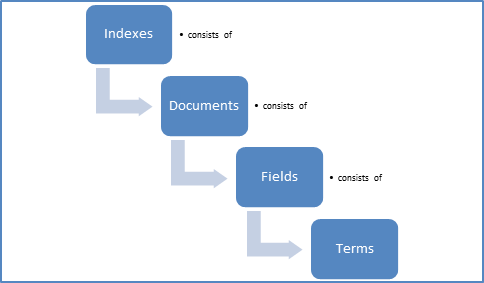
\includegraphics[width=85mm]{graph.png}

and terms are simple strings. Indexes store information about terms in order to improve search efficiency. 

We store the inverted index and the frequency with which the term appears in each document. Further as part of proximity data we also store the position where the term appears in each document along with the normalization scores used to calculate the ranking for a given query. Please note that for this blog data, we consider each blog entry as a separate instance rather than the whole blog website.
For scoring we use a combination of the Vector Space Model (VSM) of Information Retrieval \cite{baeza1999modern} and the Boolean model to determine how relevant a given Document is to a User's query. The idea behind the Vector space model is the more times a query term appears in a document relative to the number of times the term appears in the entire collection, the more relevant that document is to the query. VSM score of document d for a query q is the Cosine Similarity measure of the weighted query vectors V(q) and V(d) which can be computed as: 

cosine-similarity(q,d) = V(q) * V(d) / |V(q)| * |V(d)| 

where V(q) * V(d) is the dot product of the weighted vectors, and |V(q)| and |V(d)| are their Euclidean norms. We obtain the relevant blogs for a given query using the above, with the scores. In the rest of the paper, we augment these results with other techniques to improve the search results for the user.

We improve on the results obtained by the above technique by using the pagerank \cite{page1999pagerank}\cite{brin1998anatomy}, technique for determining the importance of blogs in the dataset. Without expanding on the idea of pagerank in detail, the intuitive idea behind the algorithm is to measure the relative importance of a page (a blog entry in this case) with respect to the entire set of documents.

In brief, given a page x which is referenced by pages t1 to tn, with O(t) as the out-degree of the page, α as the random jump factor and a graph containing total N nodes, the page rank for t can be expressed as : 

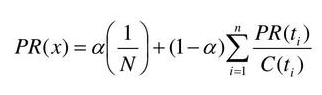
\includegraphics{eqn.png}

A point to observe here is that pagerank determines the importance of a blog irrespective of the query and hence can be augmenting with the above VSM approach to better satisfy the users information need, by reordering search results according to both criteria. In terms of implementation, dealing with a massive blog data, we have implemented an extremely optimized version of page rank in map-reduce using in-map combiners, range partitioning and combiners. We also had to partition the link graph induced from the dataset in order to be able to deal with the massive amount of data.

To combine the above techniques, we are looking at various heuristics like term weighing, re-ordering of results etc. However, at this stage we have not yet settled on the exact combining strategy which would yield optimum results for our dataset. There is an appreciable amount of literature available to best combine the orderings obtained for ranking purposes \cite{littlestone1989weighted}, like the weighted majority algorithm and we plan to implement the same. We are also experimenting with BoostingTermQuery, BoostingSpanQuery and CustomScoreQuery features provided in Lucene to encorporate the page rank evaluations while returning relevant results to the user.

The above combination of vector-space model and page rank on the original link graph of the blogs will be our baseline estimate to evaluate the users meme queries. As mentioned in the previous sections, we propose three different ways to generate the link graph after extracting memes from the data:
\begin{enumerate}
\item Using the shingling approach without grouping.
\item Using the shingling approach with grouping.
\item Using direct similarity comparisions with grouping.
\end{enumerate}

We evaluate the page rank on the graphs obtained using the three techniques above and combine them separately with the vector space model approach. Then we proceed to evaluate the returned results for a large set of users meme queries (as well as generic queries, for the sake of experimentation). We claim that we would be able to obtain much enhanced results, relevant to the users meme query using our approaches than the baseline page rank mechanism, as explained in the previous sections. We believe that in using our approaches we successfully mine richer semantics for memes, by extracting relevant memes from the blogs data, thus creating a graph which more closely models the importance of blogs for meme data.

In addition to the above techniques for evaluation, we propose to build an interface to view/interact with memes extracted by our algorithm on the blog dataset. We utilize the search engine to enable the user to perform complex queries on the dataset for obtaining the memes. As a stretch goal, we aim to enable a kind of exploratory search using a faceted interface where the user can browse the search results in an exploratory manner, thus enabling him to satisfy his information need. As a part of future work we also propose to present the memes evolution in the dataset for a specific meme query, using the temporal information available. This opens up avenues for evaluating the quality of the generated memes as well as the performance of each of the above mentioned graphs using human evaluations/mechanical turk in addition to the above experiments against the baseline approach. Finally, another opportunity is to generate a smaller synthetic dataset to analyze memes, their properties, and to determine how well our search engine and meme detection algorithm recover them. Having this smaller gold standard data, would enable us to perform experiments and retrieval precision and recall measures for our algorithm. Finally, for the sake of experimentation, we already have gold standard dataset for generic queries (non-meme) and expected results for our original dataset and it would be interesting to observe how our inferred page ranks from meme-graph compare against the baseline pagerank and the gold-standard results for those generic queries.

\section{Project Progress/Milestones}


\begin{enumerate}
  \item Preparing the data - Clean the blog dataset using Java and JQuery and convert it to JSON for further processing.	\begin{itemize}
	\item Who: Eshwaran
	\item Status: Completed
	\end{itemize}
  \item Implement substring matching using longest common substrings on mapreduce to identify common memes in pairs of blog posts. \begin{itemize}
	\item Who: Eshwaran
	\item Status: In Progress
	\end{itemize}
  \item Implement a way of computing string similarity based on various similarity measures to find common memes in pairs of blog posts.\begin{itemize}
	\item Who: Prateek
	\item Status: In Progress
	\end{itemize}
  \item Once we have the memes for the dataset, find and implement a way to group all blog posts for a given meme.\begin{itemize}
	\item Who: Eshwaran, Prateek
	\item Status: Pending
	\end{itemize}
  \item Implementation of Lucene Search Engine on raw blog data. Includes scaling to the massive dataset, inverted indexing and interface for querying.\begin{itemize}
	\item Who: Saral
	\item Status: Completed
	\end{itemize}
  \item Implement Page Rank on the original blog data using outlinks. Includes optimizations like in-mapper combining, graph partitioning and range partitioning to scale to the large dataset. \begin{itemize}
	\item Who: Saral
	\item Status: In Progress
	\end{itemize}	
  \item Implement Page Rank on the new versions of graphs generated by inferring temporal links on extracted memes. \begin{itemize}
	\item Who: Saral
	\item Status: Pending
	\end{itemize}
  \item Implement Page Rank on the new versions of graphs generated by inferring temporal links on extracted memes. \begin{itemize}
	\item Who: Saral
	\item Status: Pending
	\end{itemize}
  \item Implementation of new ranked ordering combining PageRank and Vector based models. \begin{itemize}
	\item Who: Saral
	\item Status: In Progress
	\end{itemize}
  \item Evaluation: Comparison of performance of user queries on the four approaches. Also, evaluation on generated synthetic data and on the goldstandard data available for generic queries on the blog data. \begin{itemize}
	\item Who: Eshwaran, Prateek
	\item Status: Pending
	\end{itemize}
  \item Exploratory/Faceted search over the meme results for a given user query. Also, visualizing meme evolution using temporal features in the dataset. \begin{itemize}
	\item Who: Saral
	\item Status: Pending
	\end{itemize}
\end{enumerate}

Please refer to the Pivotal Tracker generated report for detailed activity on progress


%\end{document}  % This is where a 'short' article might terminate


%
% The following two commands are all you need in the
% initial runs of your .tex file to
% produce the bibliography for the citations in your paper.
\bibliographystyle{abbrv}
\bibliography{project_progress}  % sigproc.bib is the name of the Bibliography in this case

% You must have a proper ".bib" file
%  and remember to run:
% latex bibtex latex latex
% to resolve all references
%
% ACM needs 'a single self-contained file'!
%
%APPENDICES are optional
%\balancecolumns
\end{document}
